\subsection{Senstools}
Some of the background for the implementation above comes from documentation on a Matlab toolbox called Senstools \cite{Senstools}. Since this toolbox includes an extra feature based on parameter sensitivity and frequency domain and uses Newton's method to converge faster, it is a good decision to use this tool to check the previous results.

The same data, Simulink model and initial parameters as the previous case are given to this toolbox and the result of the fit can be seen in \figref{SenseToolParameterEstimation}. 
%
\begin{figure}[H]
	\centering
	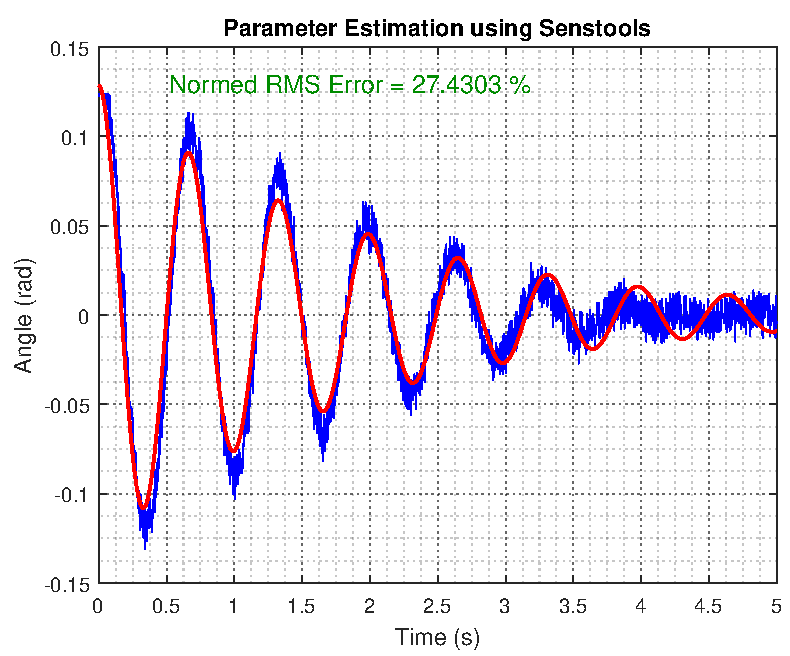
\includegraphics[scale=0.6]{figures/SenseToolParameterEstimation}
	\caption{Data from the test (red) and final fit with the new parameters (blue) made with Senstools.}
	\label{SenseToolParameterEstimation}
\end{figure}

Finally, the parameters that Senstools estimates for the model are \si{J_F=4,8 \cdot 10^{-3}\ kg \cdot m^2} and \si{B_F=7,7 \cdot 10^{-3}\ m \cdot s \cdot rad^{-1}}. The normed RMS error is \si{27,4\ \%} compared to the \si{27,54\ \%} shown in \figref{resultOfGradientWithFibonacciAndForwardBackward}. In \appref{app:ErrorComp} the normed RMS error is calculated only for the first part of the region where the fit of the graphs is best, where Senstools get \si{22,8908\ \%} and the gradient descend implementation is \si{23,0713\ \%}. It can be seen that the previously explained implementation provides a satisfactory result as the error is almost the same, but since Senstools gives a slightly better result its parameters are chosen as the final ones.

\section{Final Parameters}
The final parameters of the system can be seen in \ref{ParametersSystem}
\begin{table}[H]
	\centering
	\begin{tabular}{|l|l|p{3cm}|}
		\hline %-----------------------------------------------------------------------------------
		\textbf{Parameter} &\textbf{Value} &\textbf{Units}\\
		\hline %-----------------------------------------------------------------------------------
		\si{m_w}         & \si{0,222}       &kg\\
		\hline
		%-----------------------------------------------------------------------------------
		\si{l_w}         & \si{0,096}       &m\\
		\hline %-----------------------------------------------------------------------------------
		\si{J_w}            & \si{0,601 \cdot 10^{-3}}	&\si{kg \cdot m^2}\\
		\hline  
		%-----------------------------------------------------------------------------------
		\si{B_w}         & \si{17,03 \cdot 10^{-6}}       &N \si{\cdot m \cdot s \cdot rad^{-1}}\\
		\hline
		%-----------------------------------------------------------------------------------
		\si{m_F}         & \si{0,548}       &kg\\
		\hline
		%-----------------------------------------------------------------------------------
		\si{l_F}         & \si{0,08498}       &m\\
		\hline %-----------------------------------------------------------------------------------
		\si{J_F}            & \si{4,8 \cdot 10^{-3}}	&\si{kg \cdot m^2}\\
		\hline %-----------------------------------------------------------------------------------
		\si{B_F}         & \si{7,7 \cdot 10^{-3}}       &N \si{\cdot m \cdot s \cdot rad^{-1}}\\
		\hline
	\end{tabular}
	\caption{Parameters of the whole system.}
	\label{ParametersSystem}
\end{table}